\documentclass[11pt,letterpaper]{article}

\usepackage[letterpaper,margin=0.8in,nohead]{geometry}

\usepackage[colorlinks]{hyperref}
\usepackage{url}
\usepackage{breakurl}

\hypersetup{
	colorlinks,
	linkcolor={red},
	citecolor={red},
	urlcolor={blue}
}

\usepackage{verbatim}
\usepackage{fancyvrb}
\usepackage{scrextend}
\usepackage{enumitem}
\usepackage{url}
\usepackage{tabularx}
\usepackage[dvipsnames]{xcolor}

\usepackage{caption}
\usepackage{graphicx}
\usepackage{subcaption}

\usepackage{changepage}   % for the adjustwidth environment

\newenvironment{answer}{\em \color{blue} \begin{adjustwidth}{1cm}{1cm}}{\end{adjustwidth}}

% math
\usepackage{amsthm,amsmath}
\usepackage{amsfonts}

\newcommand{\mc}[1]{\mathcal{#1}}	% Mechanisms / Algorithms
\newcommand{\rv}[1]{\mathbf{#1}}    % Random variable

\newcommand{\pr}[1]{\mathrm{Pr}\{#1\}} % Probability

\newtheorem{corollary}{\bf Corollary}%[theorem]
\newtheorem{lemma}{\bf Lemma}%[theorem]
\newtheorem{definition}{\bf Definition}%[section]

\newtheorem{observation}{\bf Observation}%[theorem]

% load cleveref last!
\usepackage[capitalise]{cleveref}
\usepackage{float}


\begin{document}
	
	\title{EN4720: Security in Cyber-Physical Systems \\ Exercise --- Authorization}
	
	%% This is an individual assignment!!
	%% TODO: put your name and index number here here!
	\author{ \textcolor{blue}{Name: Thalagala B. P.} \\ \textcolor{blue}{Index No: 180631J}}
	
	\maketitle
	
	\begin{center}
		\color{red}\bf This is an individual exercise! \\ Due Date: 19 May 2023 by 11.59 PM
	\end{center}
	
	\vspace{1in}
	
	This exercise has to be carried out using a Linux-based PC/virtual machine. Read all the instructions and questions before attempting the exercise. Add answers under each question in the Questions section and submit the resulting PDF.
	
	\subsection*{Instructions}
	
	\begin{enumerate}
		\item Understand how linux users and groups work.
		
		\item Understand how linux file ownership and permissions work.
		
		\item Answer the questions given below.
		
	\end{enumerate}
	
	\newpage
	
	\section*{Questions}
	
%	For all the questions in this section, add a screenshot of the terminal (including all the commands you ran to perform the task) unless specified otherwise. The evaluator should be able to see each step that you followed to perform each task. In all screenshots, the areas marked (which are unique to your terminal display) in Figure 1 (the sample answer to Question 1) must be visible.
%	
%	\begin{figure}[h]
%		\centering
%		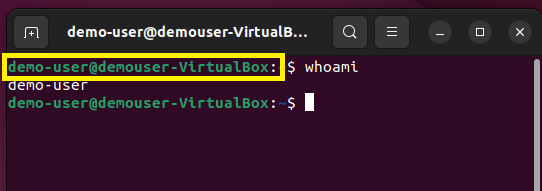
\includegraphics[width=0.65\columnwidth]{images/ex4-sample-terminal-output.png}
%		\caption{Sample Terminal Output} \label{fig:sample-terminal-output}
%	\end{figure}
	
	\begin{enumerate}
		
		\item View the currently logged in user.
		
		\begin{figure}[h]
			\centering
			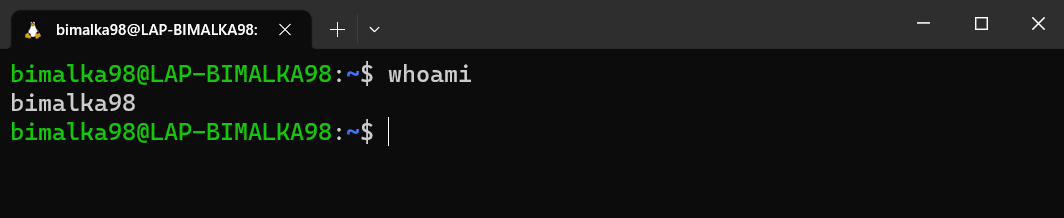
\includegraphics[width=0.65\columnwidth]{images/q1}
			\caption{Currently logged in user} \label{fig:q1}
		\end{figure}
		
		\item Create a sub directory as excercise4. Create a text file resolutions.txt with “Hello World” text in the file and store the file in the newly created directory as exercise4/resolutions.txt. Dump the file to the terminal using the \texttt{cat} command.
		
		\begin{answer}
			\begin{figure}[h]
				\centering
				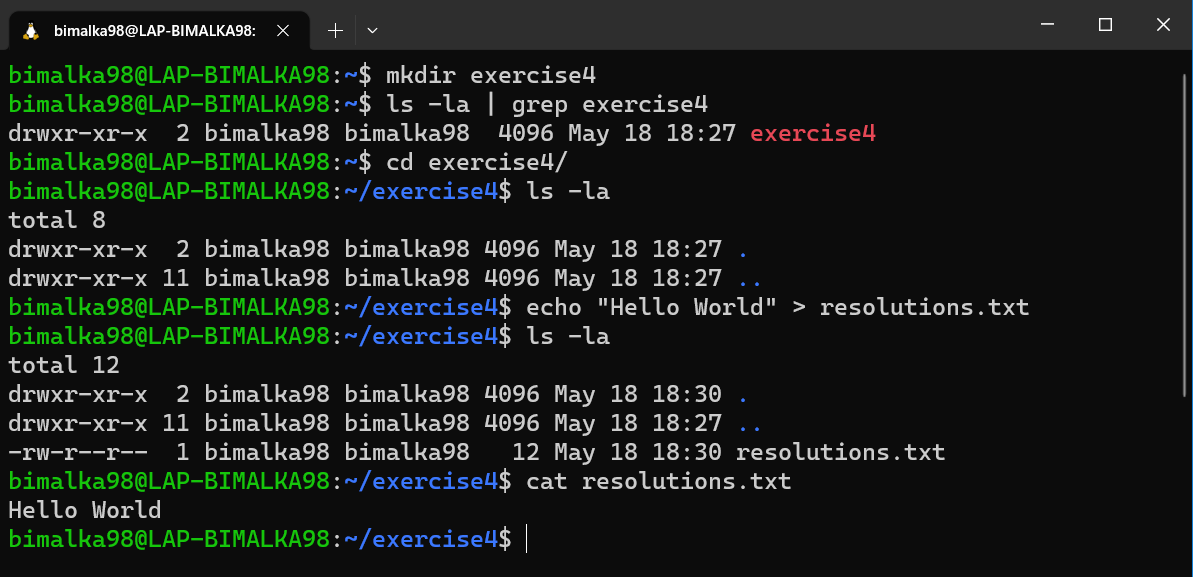
\includegraphics[width=0.65\columnwidth]{images/q2}
				\caption{Creating a sub-directory, creating a file with the required text and dump its content to the terminal} \label{fig:q2}
			\end{figure}
		\end{answer}
		
		\item Create two new user accounts as \textcolor{magenta}{alice} and \textcolor{magenta}{\textcolor{magenta}{bob}}.
		
		\begin{answer}
			\begin{figure}[h]
				\centering
				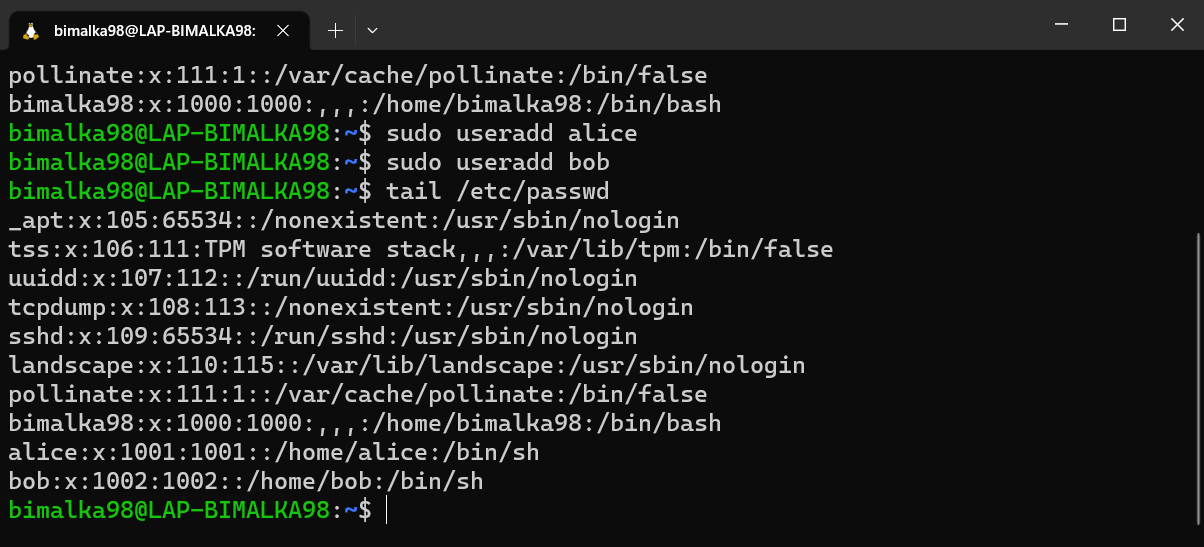
\includegraphics[width=0.65\columnwidth]{images/q3}
				\caption{Creating two new user accounts} \label{fig:q3}
			\end{figure}
		\end{answer}
		
		\item Create a group as \textcolor{ForestGreen}{friends} and add \textcolor{magenta}{alice} and yourself (currently logged in user) to the group \textcolor{ForestGreen}{friends}
		
		\begin{answer}
			\begin{figure}[H]
				\centering
				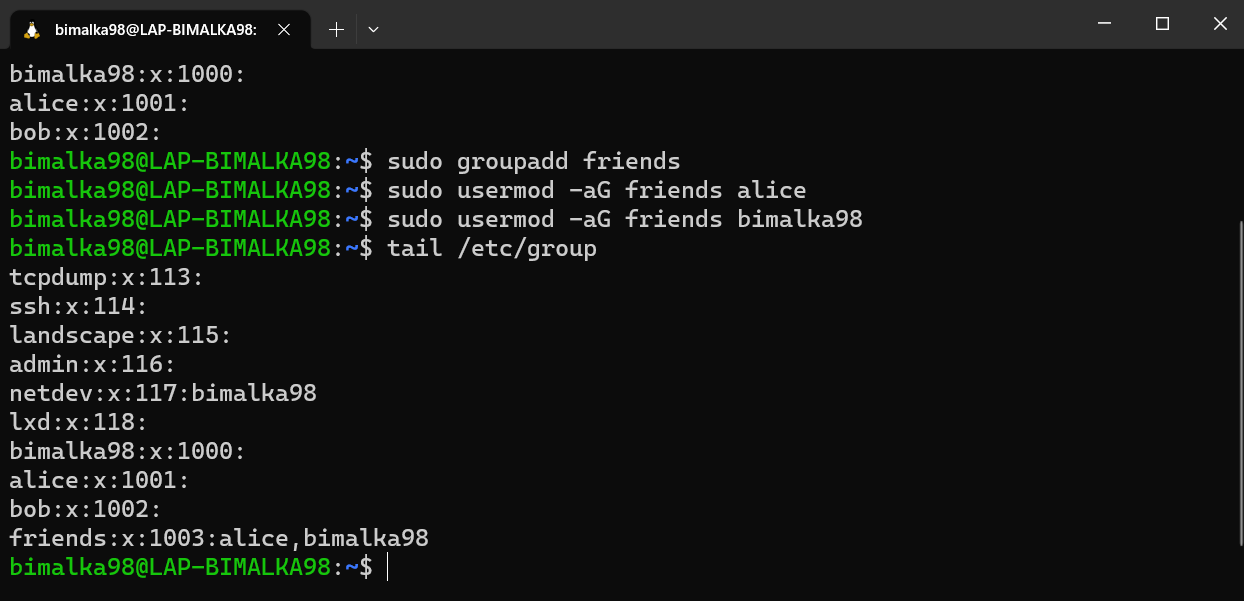
\includegraphics[width=0.65\columnwidth]{images/q4}
				\caption{Creating a group and add members} \label{fig:q4}
			\end{figure}
		\end{answer}
		
		\item Make sure your (currently logged in user's) home directory has execute permissions for all the users.
		
		\begin{answer}
			\begin{figure}[H]
				\centering
				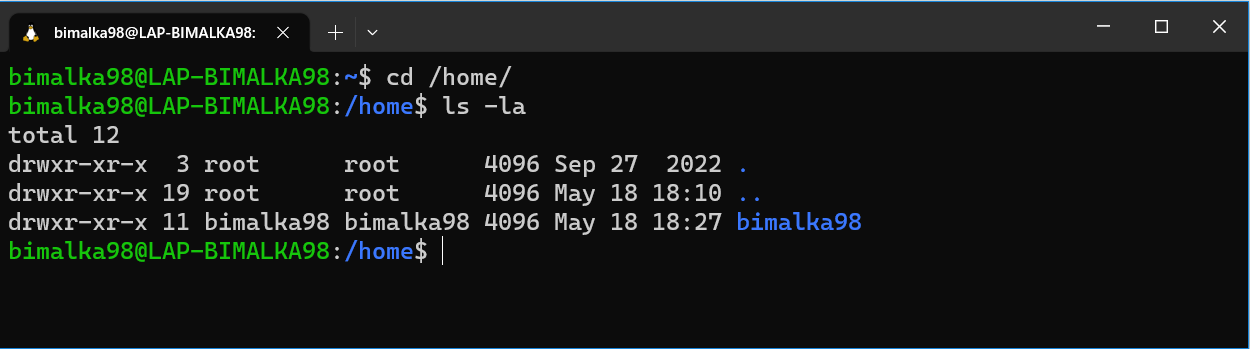
\includegraphics[width=0.65\columnwidth]{images/q5}
				\caption{Execution permission to the current user's home directory} \label{fig:q5}
			\end{figure}
		\end{answer}
		\pagebreak
		\item Become (log in as) one of your new user accounts (\textcolor{magenta}{alice} or \textcolor{magenta}{bob}). You can simply \texttt{su -} to the alternate user.
		
		\begin{answer}
			\begin{figure}[H]
				\centering
				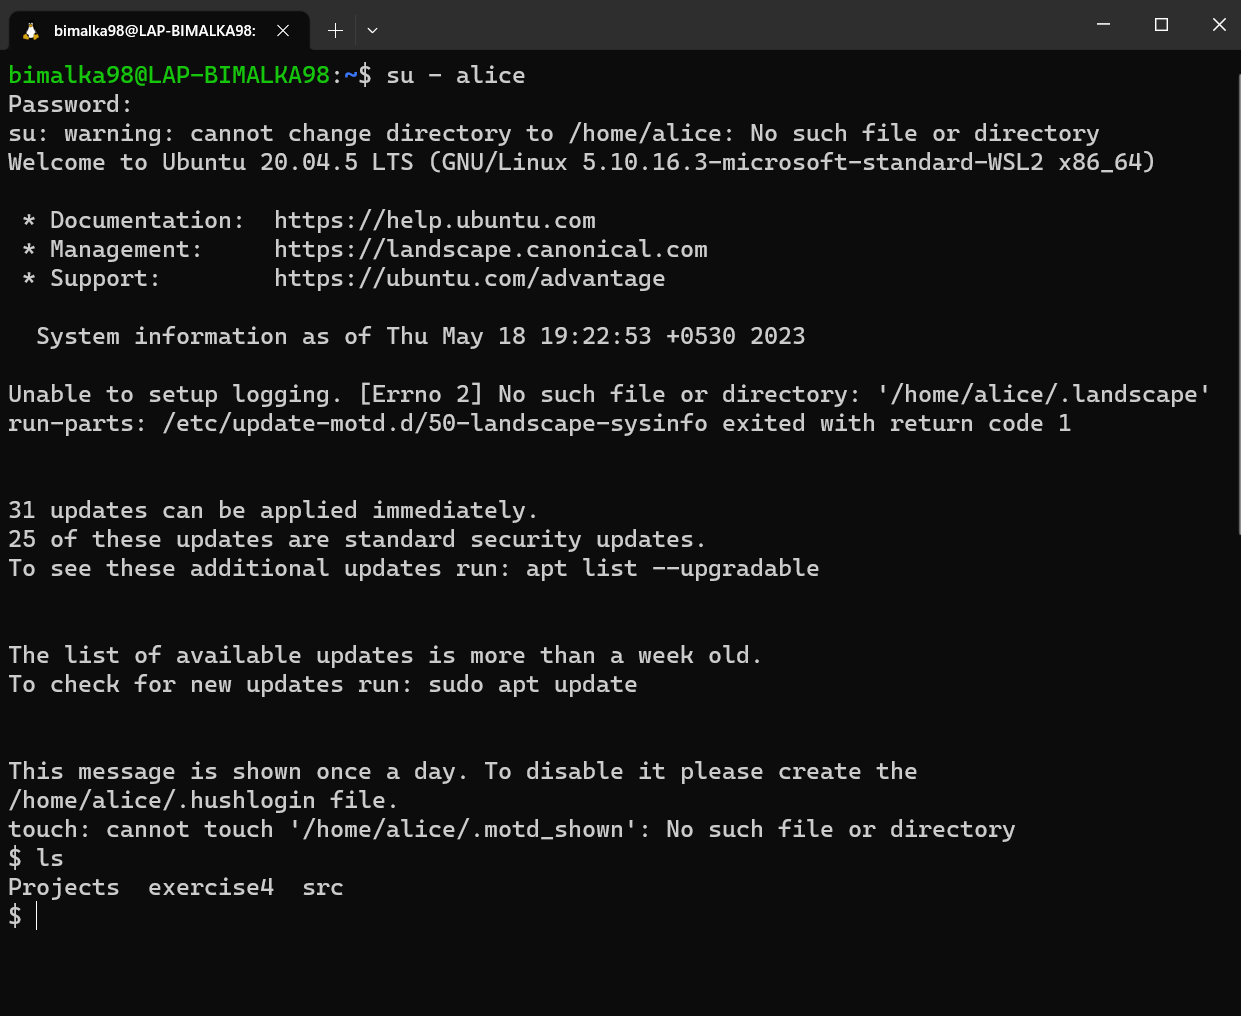
\includegraphics[width=0.65\columnwidth]{images/q6}
				\caption{Log-in as the user {\tt alice}} \label{fig:q6}
			\end{figure}
		\end{answer}
		
		
		\item As the new user, confirm that you can view the file by dumping the content to the terminal. Try adding a new item to the resolutions.txt file. Why can’t you modify the file as the new user?
		
		\begin{answer}
			\begin{figure}[H]
				\centering
				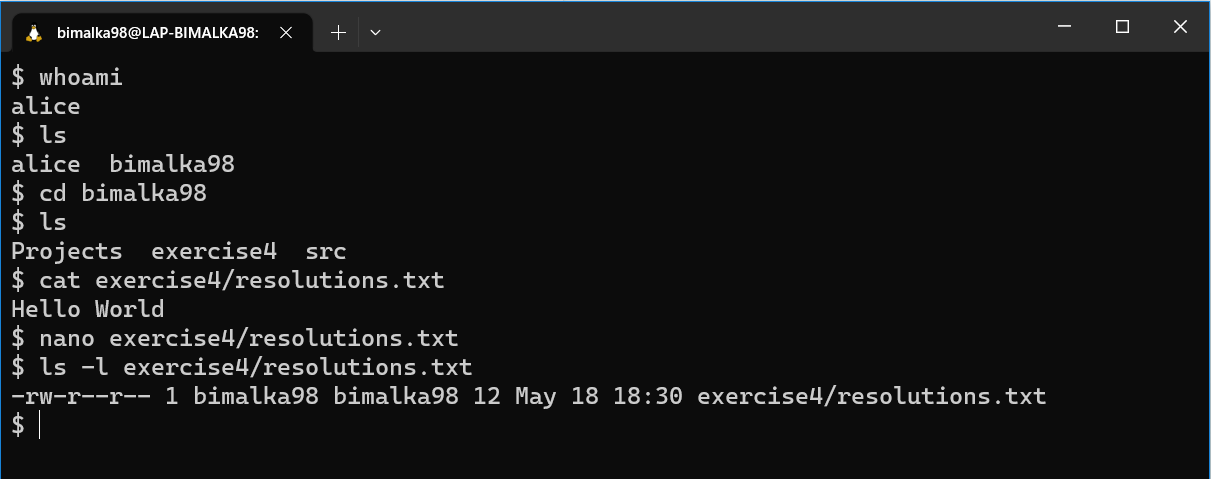
\includegraphics[width=0.65\columnwidth]{images/q7_1}
				\caption{Viewing the content of the {\tt resolutions.txt} file} \label{fig:q7_1}
			\end{figure}
		
		As the Figure \ref{fig:q7_2} illustrates, altering the content of the {\tt resolutions.txt} file, is denied. Because, the {\tt other} users in the Linux host machine has only the {\tt read}  permission for that file, and no write permission is given to them. This fact is verified by the output of the last command in the Figure \ref{fig:q7_1}, which inspects various permissions to the {\tt resolutions.txt} file. The line segment {\tt -rw-r--r--} indicates that the User {\tt bimalka98} has Read and Write permissions (rw-), the Group {\tt bimalka98} has Read permission (r--), and Others have Read permission (r--).

		
			\begin{figure}[H]
				\centering
				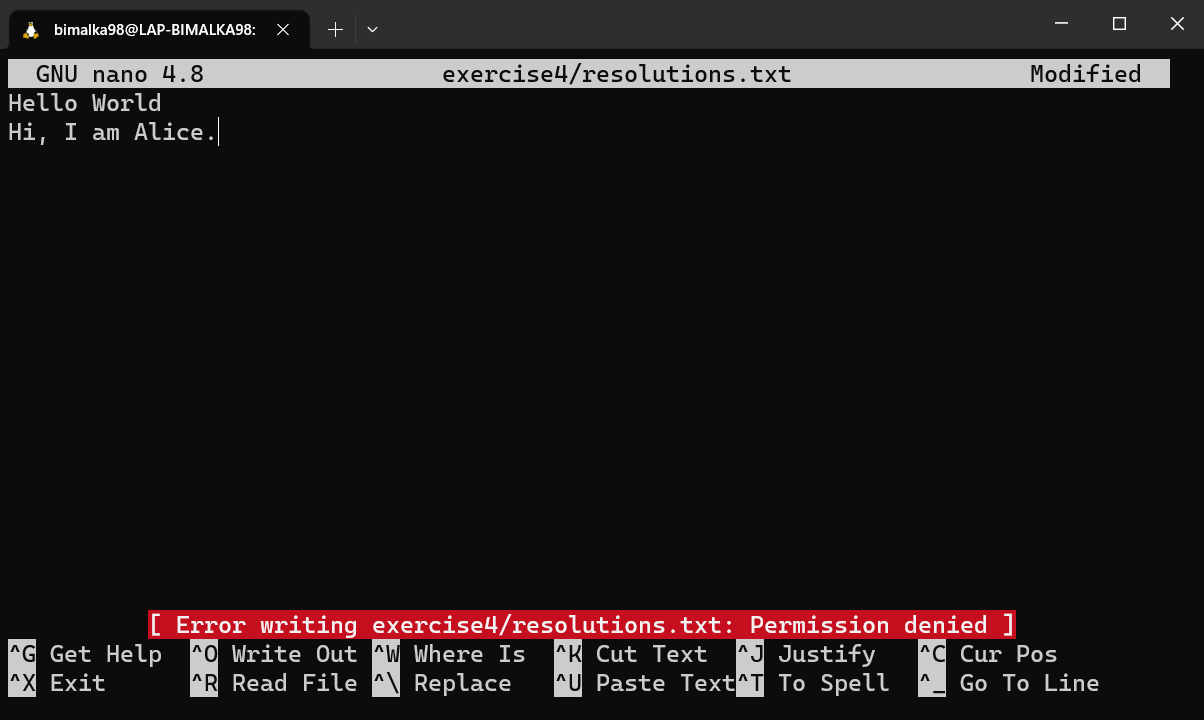
\includegraphics[width=0.65\columnwidth]{images/q7_2}
				\caption{Trying to alter the content of the {\tt resolutions.txt} file: Permission Denied.} \label{fig:q7_2}
			\end{figure}
		\end{answer}
		
		\item Note that the permissions on a newly created file allow all users on the system to read the file. Assume that you want to keep resolutions.txt file private. Modify the file's permissions, such that read access for others is removed. 
		
		\begin{answer}
			\begin{figure}[H]
				\centering
				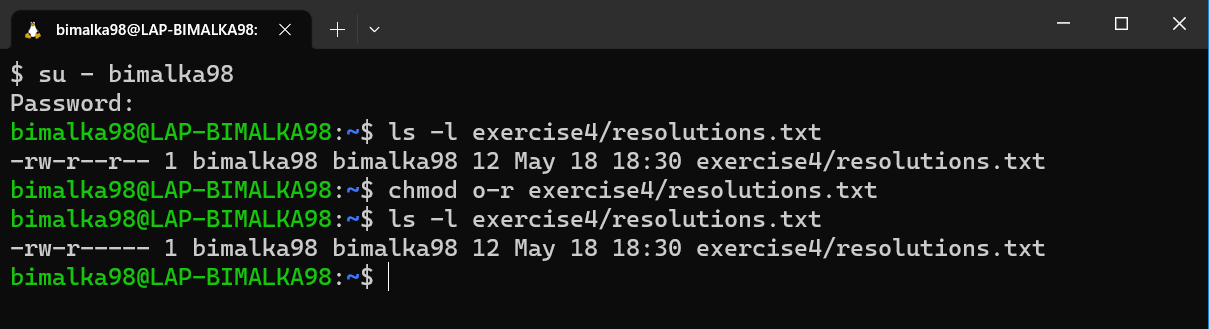
\includegraphics[width=0.65\columnwidth]{images/q8}
				\caption{Removing the read access for {\tt other} users} \label{fig:q8}
			\end{figure}
		\end{answer}
		
		
		\item Using the other new account (if you used \textcolor{magenta}{alice} before, now use \textcolor{magenta}{bob}), confirm that other users on the system are not able to read your resolutions.txt file by trying to dump the file to the terminal.
		
		\begin{answer}
			\begin{figure}[H]
				\centering
				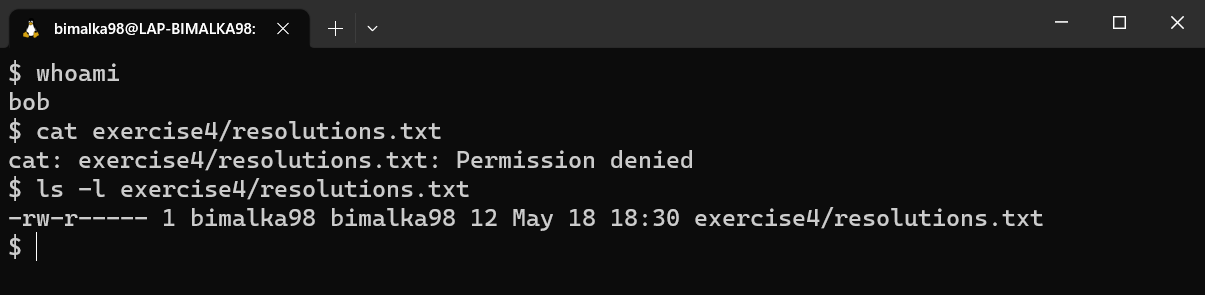
\includegraphics[width=0.65\columnwidth]{images/q9}
				\caption{Confirming that other users on the system are not able to read your {\tt resolutions.txt} file, by trying to viewing its content from bob's account} \label{fig:q9}
			\end{figure}
		\end{answer}
		
		\pagebreak
		\item Compose a short shopping list in your preferred text editor, or using the command line. Store the file as exercise4/shopping.txt. Change the group owner of the file to \textcolor{ForestGreen}{friends}.
		
		\begin{answer}
			\begin{figure}[H]
				\centering
				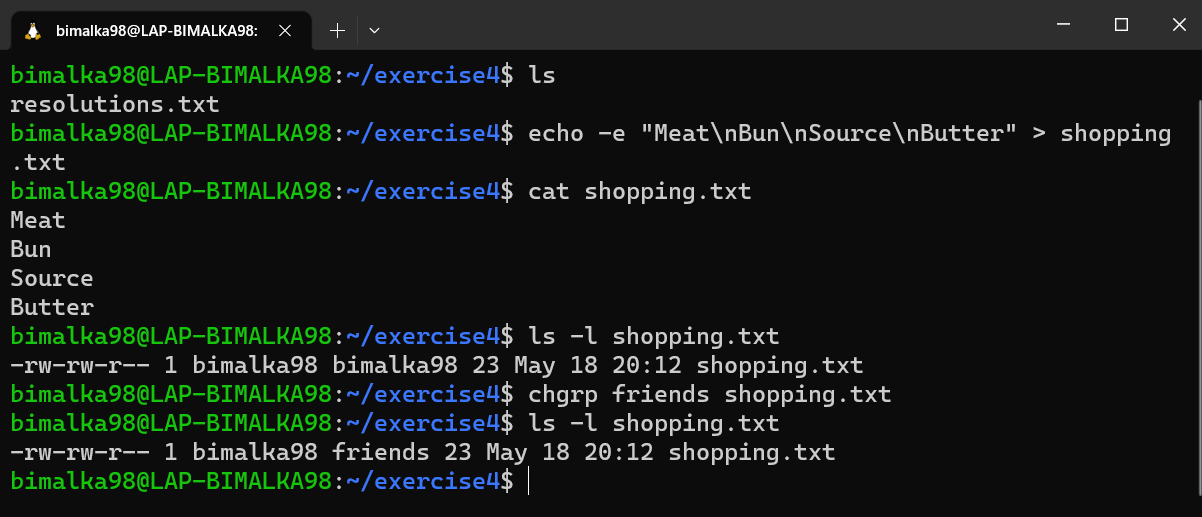
\includegraphics[width=0.65\columnwidth]{images/q10}
				\caption{Creating the {\tt shopping.txt} file and change its group owner} \label{fig:q10}
				\end{figure}
		\end{answer}
		
		\item As the alternate user \textcolor{magenta}{alice}, confirm that you can view the file. Also, note that you can modify the file, by adding an additional item to the shopping list. Dump the file content to the terminal to show that the new item is added.
		
		\begin{answer}
			\begin{figure}[H]
				\centering
				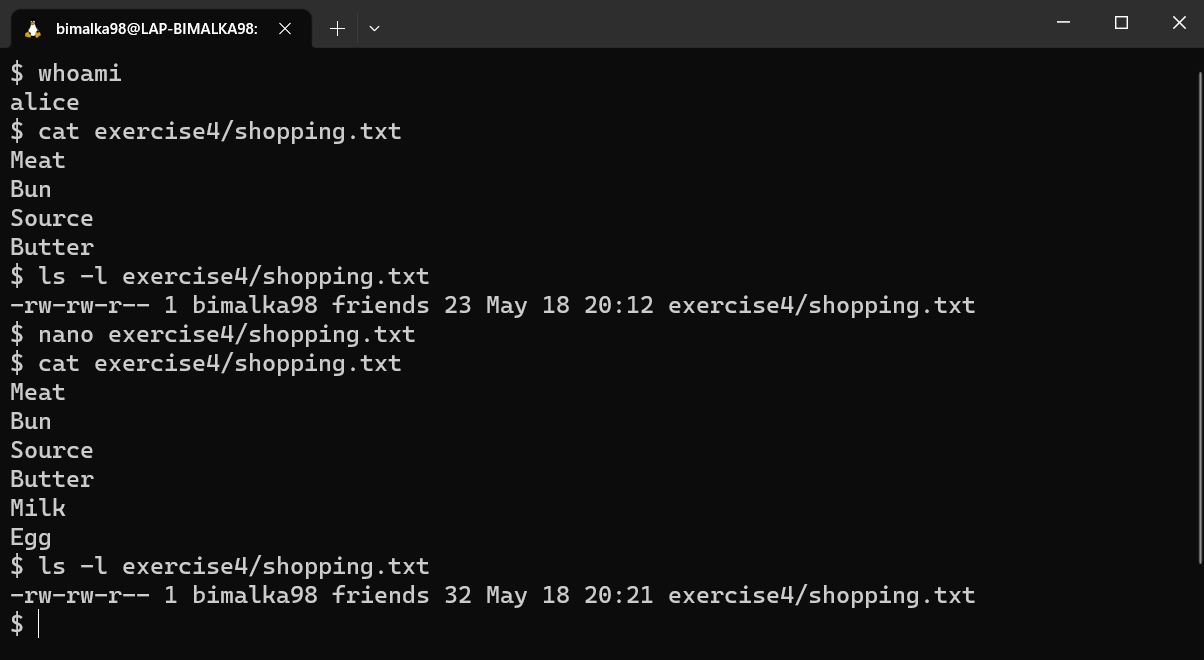
\includegraphics[width=0.65\columnwidth]{images/q11_1}
				\caption{Confirming the read and write permission of the users of the friends group} \label{fig:q11_1}
			\end{figure}
		\end{answer}
		\pagebreak
		\item Recall that your other new account (\textcolor{magenta}{bob}) is not a member of the group \textcolor{ForestGreen}{friends}. Try becoming \textcolor{magenta}{bob} and repeat the previous steps. You should be able to view, but not modify, the file.
		
		\begin{answer}
		\begin{figure}[H]
			\centering
			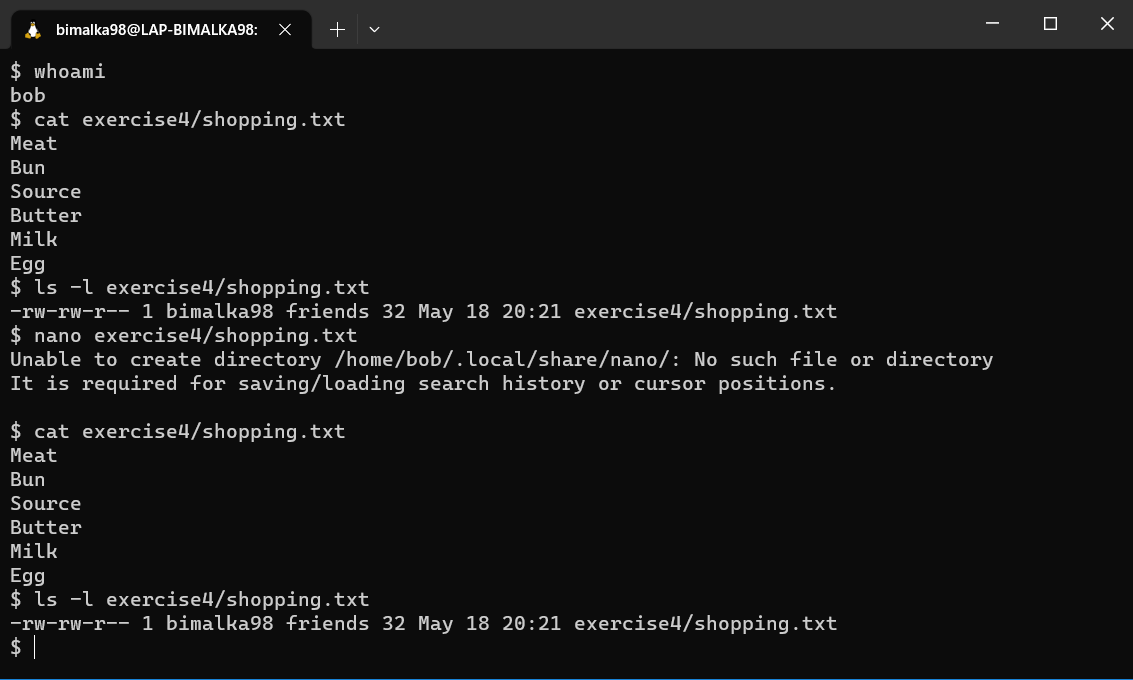
\includegraphics[width=0.65\columnwidth]{images/q12_1}
			\caption{Checking the read and write permission of the user {\tt bob}} \label{fig:q12_1}
		\end{figure}
	
		\begin{figure}[H]
			\centering
			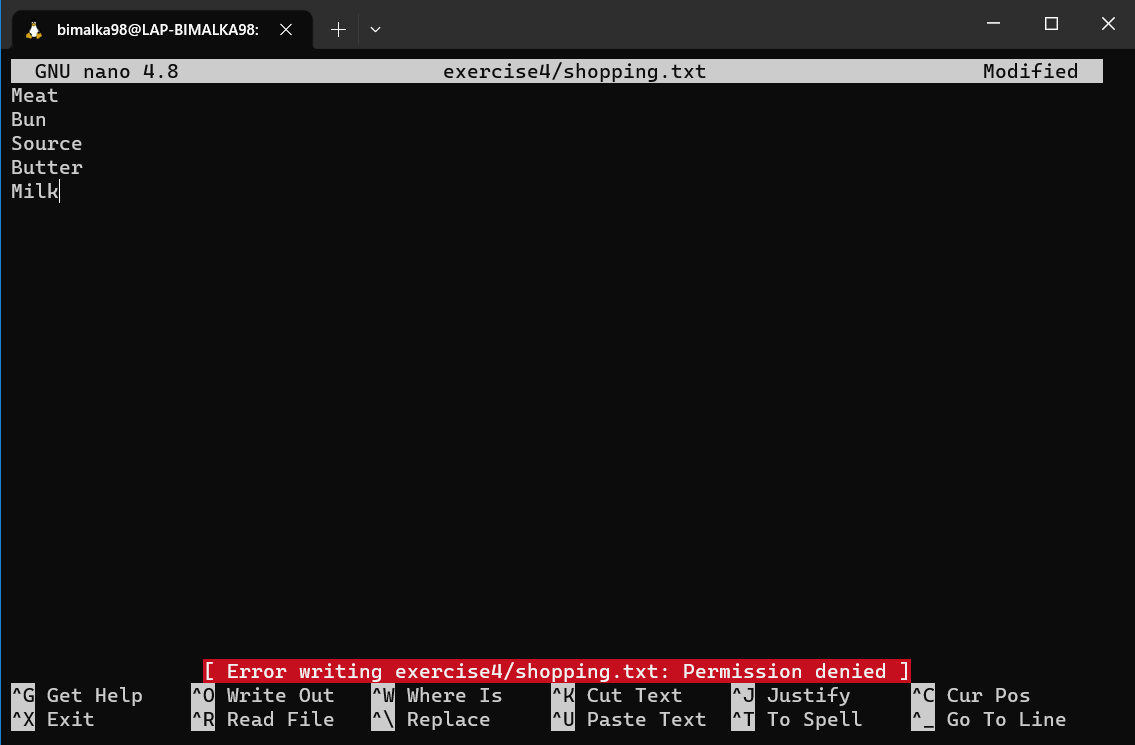
\includegraphics[width=0.65\columnwidth]{images/q12_2}
			\caption{Verifying the user {\tt bob} does not have write permission} \label{fig:q12_2}
		\end{figure}
		\end{answer}
		
		\vspace{5mm}
		\pagebreak
		Provide analytical answers to the questions below. Screenshots are not required.
		
		\item What are the challenges that organizations face during the cyber security authorization process, and how can they be overcome?				
		
		\begin{answer}
		The following answer was adopted from \url{https://www.accenture.com/us-en/blogs/security/keys-successful-access-authorization}
		
		Challenges and ways to overcome them:
		\begin{itemize}
			\item \textbf{Lack of vendor solutions} - Due to inflexibility and performance concerns of the available cyber security authorization processes, most organizations chose to build the authorization systems which best suits for their specific requirement. The growth of the number of vendor specializing in this area is a way to overcome this challenge. So that organization can select the best match for their requirements and adopt the solution accordingly.  

			\item \textbf{Complexity of managing policies} - When managing authorization processes, organizations need to maintain/ update rules that determine who is allowed to access certain information and resources. This process involve, analyzing the existing complex code to identify already existing rules and reverse engineer the existing decision making (if/ else) algorithms to understand how those rules are enforced. This whole process is super complex to carry out manually.Tools with Artificial Intelligence capabilities have been built by vendors to dynamically generate and manage policies. In addition to that friendly user interfaces that hides the complexity of extensible access control markup language (XACML) has also become a grate relief.
			
			
			\item \textbf{Performance and scale} - Organizations need to make sure that their systems can handle the ever increasing demands of the authorization process. However, this process involves communication between various system components which essentially can slow down the system. Focusing on modernizing applications and systems that take advantage of cloud technologies is a way to address this issue, as they often have better integration with authorization tools.
		\end{itemize}
		
		\end{answer}
		
		\item How do different cyber security authorization frameworks differ from one another, and what are the key considerations that organizations should take into account when choosing a framework to follow?
		
		\begin{answer}
			The following answer was adopted from \url{https://www.knowledgehut.com/blog/security/cyber-security-frameworks}
			
			Key considerations that organizations should take into account when choosing a framework to follow:
			\begin{itemize}
				\item 
			\end{itemize}
		\end{answer}
		
		\item What are the most common vulnerabilities that may be identified during the cyber security authorization process, and how can organizations address them?
		
		\begin{answer}
			%% TODO: Add answer here
			Your answer here
		\end{answer}
		
	\end{enumerate}
	
\end{document}